\documentclass{beamer}
\usepackage[utf8]{inputenc}
\usepackage{amsmath}
\usepackage{amssymb}
\usepackage{xcolor}
\usepackage{hyperref}
\usepackage{listings}
\usepackage{graphicx}

\usetheme{Madrid}
\usecolortheme{default}

\title{Applying Deep Learning to Inverse Kinematics}
\author{Nathan Hersch}
\date{\today}

% Define code style
\lstset{
    basicstyle=\ttfamily\small,
    breaklines=true,
    columns=fullflexible,
    showstringspaces=false,
    commentstyle=\color{gray},
    keywordstyle=\color{blue},
    stringstyle=\color{red},
    language=Python
}

\begin{document}

\frame{\titlepage}

\begin{frame}{Outline}
    \tableofcontents
\end{frame}

\section{Universal Approximation Theorem}

\begin{frame}{Universal Approximation Theorem}
    \begin{block}{Core Principle}
        Universal approximation theorem proves that for any continuous function, there exists a network that can approximate this function to any specified precision.
    \end{block}
    
    \vspace{0.5cm}
    
    \begin{center}
        \includegraphics[width=0.7\textwidth]{uat.png}
    \end{center}
    
    \vspace{0.3cm}
    
    \small \textit{This theorem provides the theoretical foundation for using neural networks to learn inverse kinematics.}
\end{frame}

\section{Robotics Kinematics}

\begin{frame}{Robotic Manipulators}
    \begin{columns}
        \column{0.5\textwidth}
        \centering
        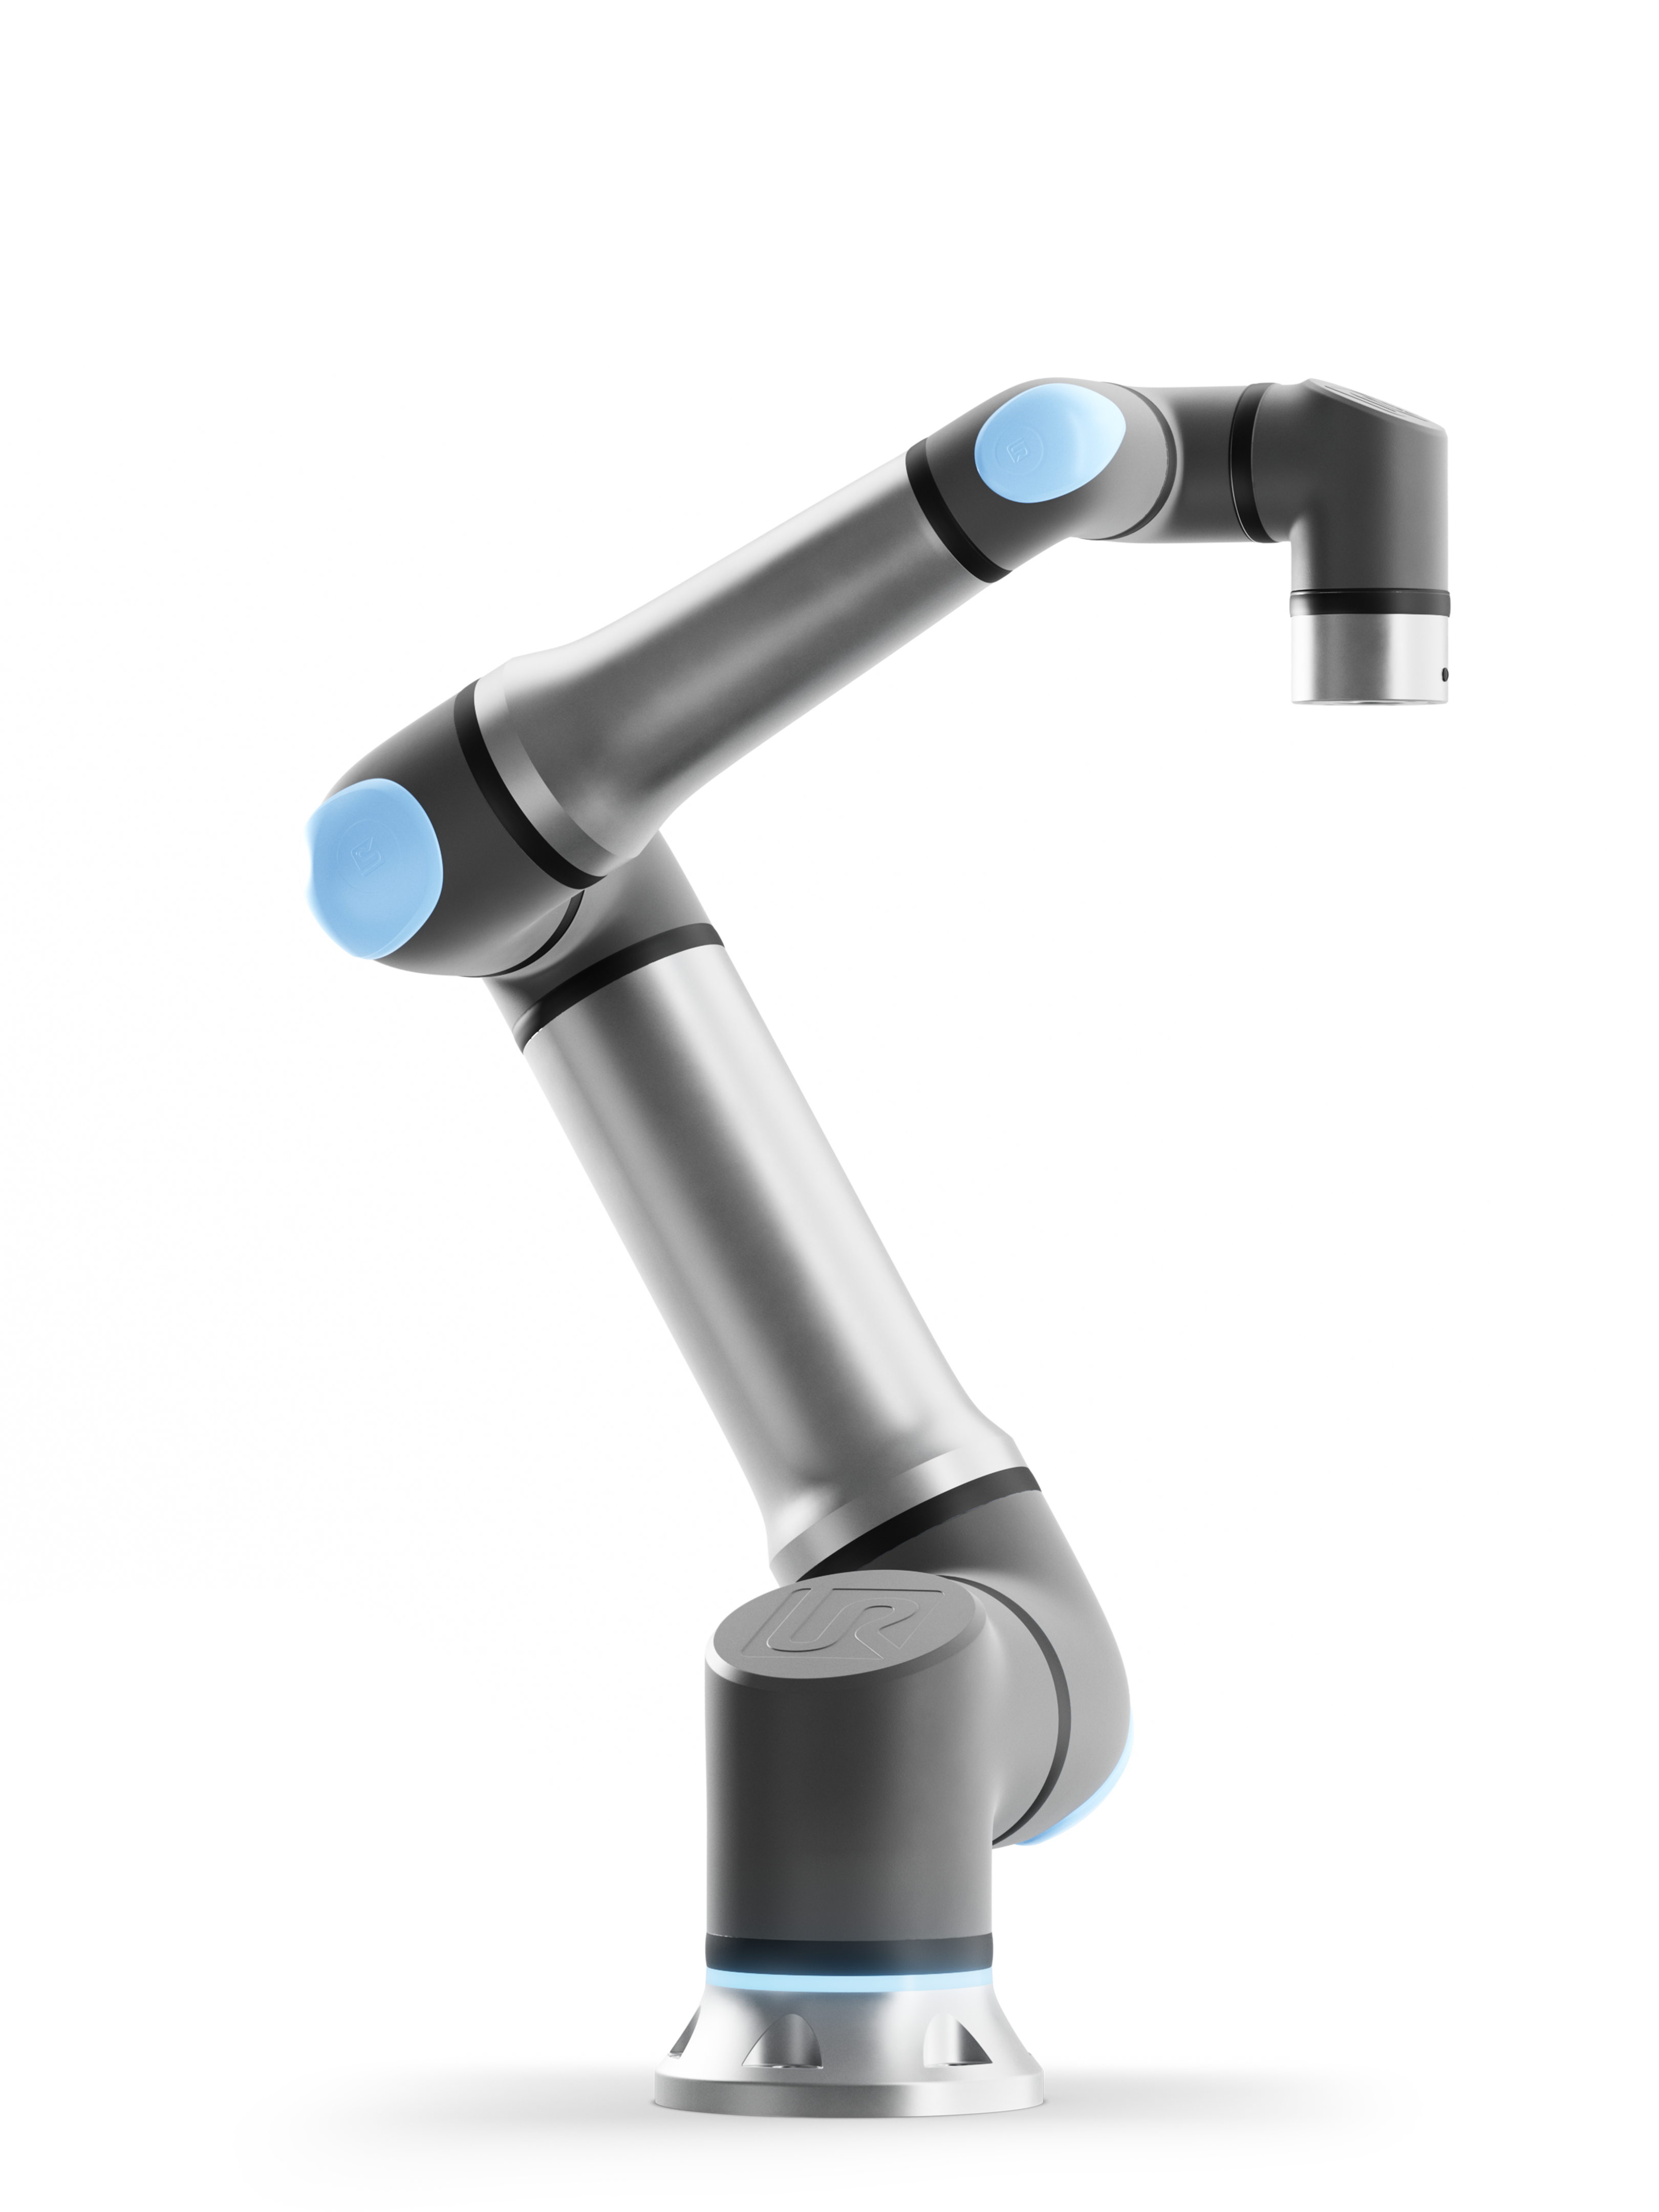
\includegraphics[width=\textwidth]{ur.png}
        
        \textbf{Universal Robot (UR)}
        
        \column{0.5\textwidth}
        \centering
        \includegraphics[width=\textwidth]{scara.png}
        
        \textbf{SCARA Robot}
    \end{columns}
    
    \vspace{0.8cm}
    
    \textit{Different robot configurations require different kinematic solutions}
\end{frame}

\begin{frame}{Two-Link Planar Manipulator}
    \begin{columns}
        \column{0.5\textwidth}
        \includegraphics[width=\textwidth]{2link.png}
        
        \column{0.5\textwidth}
        \textbf{Problem Setup:}
        \begin{itemize}
            \item Link lengths: $a_1, a_2$
            \item Joint angles: $\theta_1, \theta_2$
            \item End-effector: $(x, y)$
        \end{itemize}
        
        \vspace{0.3cm}
        
        \small Simple case to understand forward and inverse kinematics
    \end{columns}
\end{frame}

\begin{frame}{Forward Kinematics (2-Link)}
    \textbf{From geometry of the two revolute links:}
    
    \begin{equation}
    x = a_1 \cos\theta_1 + a_2 \cos(\theta_1 + \theta_2)
    \end{equation}
    
    \begin{equation}
    y = a_1 \sin\theta_1 + a_2 \sin(\theta_1 + \theta_2)
    \end{equation}
    
    \vspace{0.5cm}
    
    \textbf{Interpretation:}
    \begin{itemize}
        \item Given: Joint angles $\theta_1, \theta_2$
        \item Compute: End-effector position $(x, y)$
        \item Direct and unambiguous calculation
    \end{itemize}
\end{frame}

\begin{frame}{Inverse Kinematics (2-Link) --- Step 1}
    \textbf{Step 1: Solve for $\theta_2$ (elbow angle)}
    
    \vspace{0.3cm}
    
    Define: $r^2 = x^2 + y^2$
    
    \vspace{0.3cm}
    
    Apply law of cosines:
    \begin{equation}
    \cos\theta_2 = \frac{r^2 - a_1^2 - a_2^2}{2a_1 a_2}
    \end{equation}
    
    \vspace{0.3cm}
    
    Solve for angle:
    \begin{equation}
    \theta_2 = \text{atan2}\left(\pm\sqrt{1 - \cos^2\theta_2}, \cos\theta_2\right)
    \end{equation}
    
    \vspace{0.3cm}
    
    \textbf{Note:}
    \begin{itemize}
        \item The $\pm$ gives two solutions: ``elbow-down'' and ``elbow-up''
        \item This is the \textit{multiple solutions problem}
    \end{itemize}
\end{frame}

\begin{frame}{Inverse Kinematics (2-Link) --- Step 2}
    \textbf{Step 2: Solve for $\theta_1$ (shoulder angle)}
    
    \vspace{0.3cm}
    
    Using the shoulder and elbow geometry:
    \begin{equation}
    \theta_1 = \text{atan2}(y, x) - \text{atan2}\left(a_2\sin\theta_2, a_1 + a_2\cos\theta_2\right)
    \end{equation}
    
    \vspace{0.5cm}
    
    \textbf{Result:}
    \begin{itemize}
        \item We now have the joint angles that place end-effector at $(x, y)$
        \item Two possible configurations exist (elbow-down, elbow-up)
        \item This is the classic geometric IK solution for planar 2-DOF robots
    \end{itemize}
    
    \vspace{0.3cm}
    
    \small \textit{For complex robots, we need a general framework...}
\end{frame}

\section{Denavit-Hartenberg Parameters}

\begin{frame}{Denavit-Hartenberg (DH) Parameterization}
    \begin{block}{DH Parameter Convention}
        A standard method to describe robot geometry using 4 parameters per joint:
        \begin{itemize}
            \item $a_i$: link length (distance along $\hat{x}$-axis)
            \item $d_i$: link offset (distance along $\hat{z}$-axis)
            \item $\alpha_i$: link twist (rotation around $\hat{x}$-axis)
            \item $\theta_i$: joint angle (rotation around $\hat{z}$-axis)
        \end{itemize}
    \end{block}
    
    \vspace{0.5cm}
    
    \textbf{Note:} Either $d_i$ or $\theta_i$ can be variable depending on joint type. For ease of explanation, we will only use $\theta_i$ as the variable (revolute joints).
\end{frame}

\begin{frame}{Homogeneous Transformation Matrix}
    \textbf{The transformation is represented as a product of four basic transformations:}
    
    \begin{equation*}
    A_i = \text{Rot}_{z,\theta_i} \cdot \text{Trans}_{z,d_i} \cdot \text{Trans}_{x,a_i} \cdot \text{Rot}_{x,\alpha_i}
    \end{equation*}
    
    \vspace{0.3cm}
    
    \tiny
    \begin{equation*}
    = \begin{bmatrix}
    c_{\theta_i} & -s_{\theta_i} & 0 & 0 \\
    s_{\theta_i} & c_{\theta_i} & 0 & 0 \\
    0 & 0 & 1 & 0 \\
    0 & 0 & 0 & 1
    \end{bmatrix}
    \begin{bmatrix}
    1 & 0 & 0 & 0 \\
    0 & 1 & 0 & 0 \\
    0 & 0 & 1 & d_i \\
    0 & 0 & 0 & 1
    \end{bmatrix}
    \begin{bmatrix}
    1 & 0 & 0 & a_i \\
    0 & 1 & 0 & 0 \\
    0 & 0 & 1 & 0 \\
    0 & 0 & 0 & 1
    \end{bmatrix}
    \begin{bmatrix}
    1 & 0 & 0 & 0 \\
    0 & c_{\alpha_i} & -s_{\alpha_i} & 0 \\
    0 & s_{\alpha_i} & c_{\alpha_i} & 0 \\
    0 & 0 & 0 & 1
    \end{bmatrix}
    \end{equation*}
    
    \vspace{0.3cm}
    
    \normalsize
    \begin{equation*}
    A_i = \begin{bmatrix}
    c_{\theta_i} & -s_{\theta_i}c_{\alpha_i} & s_{\theta_i}s_{\alpha_i} & a_i c_{\theta_i} \\
    s_{\theta_i} & c_{\theta_i}c_{\alpha_i} & -c_{\theta_i}s_{\alpha_i} & a_i s_{\theta_i} \\
    0 & s_{\alpha_i} & c_{\alpha_i} & d_i \\
    0 & 0 & 0 & 1
    \end{bmatrix}
    \end{equation*}
    
    \small Where $c_{\theta_i} = \cos\theta_i$ and $s_{\theta_i} = \sin\theta_i$
\end{frame}

\begin{frame}{RRR Robot Architecture (3-DOF)}
    \textbf{RRR Configuration:} Three revolute joints
    
    \vspace{0.3cm}
    
    DH Parameters:
    \begin{table}
        \centering
        \small
        \begin{tabular}{|c|c|c|c|c|}
            \hline
            Joint & $a_i$ (mm) & $d_i$ (mm) & $\alpha_i$ & $\theta_i$ (variable) \\
            \hline
            1 & 0 & 0 & $-90^\circ$ & $\theta_1$ \\
            2 & 0 & 0 & $+90^\circ$ & $\theta_2$ \\
            3 & 0 & 50 & $0^\circ$ & $\theta_3$ \\
            \hline
        \end{tabular}
    \end{table}
    
    \vspace{0.3cm}
    
    \textbf{Workspace:}
    \begin{itemize}
        \item 3 DOF allows positioning in 3D space
        \item Multiple configurations possible (redundancy)
        \item Used as primary test case
    \end{itemize}
\end{frame}

\begin{frame}{RRRRRR Robot Architecture (6-DOF)}
    \textbf{RRRRRR Configuration:} Six revolute joints
    
    \vspace{0.3cm}
    
    DH Parameters:
    \begin{table}
        \centering
        \tiny
        \begin{tabular}{|c|c|c|c|}
            \hline
            Joint & $a_i$ & $d_i$ & $\alpha_i$ \\
            \hline
            1 & 0 & 0 & $-90^\circ$ \\
            2 & 0 & 0 & $+90^\circ$ \\
            3 & 0 & 50 & $0^\circ$ \\
            4 & 0 & 100 & $-90^\circ$ \\
            5 & 0 & 0 & $+90^\circ$ \\
            6 & 0 & 50 & $0^\circ$ \\
            \hline
        \end{tabular}
    \end{table}
    
    \vspace{0.2cm}
    
    \textbf{Characteristics:}
    \begin{itemize}
        \item 6 degrees of freedom (full pose control)
        \item More complex workspace geometry
        \item Higher dimensional solution space
    \end{itemize}
\end{frame}

\section{Classical Solutions}

\begin{frame}{Classical Geometric Solution}
    \textbf{Approach:} Decompose problem into geometric subproblems
    
    \vspace{0.3cm}
    
    \textbf{Advantages:}
    \begin{itemize}
        \item Algebraically exact solutions
        \item Computationally fast ($\sim 1\,\mu\text{s}$)
        \item Deterministic
    \end{itemize}
    
    \vspace{0.3cm}
    
    \textbf{Disadvantages:}
    \begin{itemize}
        \item Problem-specific (doesn't generalize)
        \item Requires expert knowledge of robot geometry
        \item Difficult for 6+ DOF systems
        \item May miss some solutions
    \end{itemize}
\end{frame}

\begin{frame}{Damped Least Squares (DLS) Method}
    \textbf{Iterative Approach:} Refine joint angles to minimize pose error
    
    \vspace{0.3cm}
    
    \textbf{DLS Update Rule:}
    \begin{equation*}
    \Delta\theta = (J^T J + \lambda^2 I)^{-1} J^T \mathbf{e}
    \end{equation*}
    
    Where:
    \begin{itemize}
        \item $J$: Jacobian matrix --- $\frac{\partial FK(\theta)}{\partial \theta}$
        \item $\mathbf{e}$: pose error vector --- $\mathbf{e} = p_{\text{target}} - FK(\theta_{\text{current}})$
        \item $\lambda$: damping factor (prevents singular matrices, typically $0.01\text{--}0.1$)
    \end{itemize}
    
    \vspace{0.3cm}
    
    \textbf{Algorithm:}
    \begin{enumerate}
        \item Initialize: $\theta_0 = [0, 0, 0, \ldots]$
        \item Compute: $\mathbf{e} = p_{\text{target}} - FK(\theta)$ and Jacobian $J$
        \item Update: $\theta \leftarrow \theta + \Delta\theta$
        \item Repeat until: $\|\mathbf{e}\| < \epsilon$ (e.g., $\epsilon = 10^{-6}$ rad)
    \end{enumerate}
\end{frame}

\begin{frame}{DLS Method Characteristics}
    \textbf{Convergence Properties:}
    \begin{itemize}
        \item Typically converges in 10--100 iterations
        \item Each iteration: $\sim 100\,\mu\text{s}$ (depends on DOF)
        \item Total time: $\sim 1\text{--}10\,\text{ms}$ per IK solution
    \end{itemize}
    
    \vspace{0.5cm}
    
    \textbf{Advantages:}
    \begin{itemize}
        \item General method (works for any robot)
        \item Handles singularities through damping
        \item Approximate but converges reliably
    \end{itemize}
    
    \vspace{0.5cm}
    
    \textbf{Disadvantages:}
    \begin{itemize}
        \item Slower than geometric solutions
        \item May converge to local minimum
        \item Requires good initial guess
        \item Not suitable for real-time control at high frequencies
    \end{itemize}
\end{frame}

\section{Universal Approximation Applied to IK}

\begin{frame}{Why Neural Networks for IK?}
    \begin{block}{Key Insight}
        Since inverse kinematics is a mapping from $(x, y, z, \text{roll}, \text{pitch}, \text{yaw})$ to joint angles $(\theta_1, \theta_2, \ldots, \theta_n)$, this should be something that we can use universal approximation theorem to learn.
    \end{block}
    
    \vspace{0.5cm}
    
    \textbf{IK as a Function:}
    \begin{equation*}
    f: \mathbb{R}^6 \rightarrow \mathbb{R}^n
    \end{equation*}
    \begin{equation*}
    (x, y, z, r, p, y) \mapsto (\theta_1, \theta_2, \ldots, \theta_n)
    \end{equation*}
    
    \vspace{0.5cm}
    
    \textbf{If we can learn this mapping:}
    \begin{itemize}
        \item No iterative solving required
        \item Single forward pass through network
        \item Potential for real-time performance
    \end{itemize}
\end{frame}

\section{The Problem: Multiple IK Solutions}

\begin{frame}[fragile]{Dataset Generation Method}
    \textbf{Our Approach:} Generate random joint angles, compute forward kinematics
    
    \vspace{0.3cm}
    
    \begin{lstlisting}[basicstyle=\ttfamily\tiny]
def generate_consistent_dataset(dh_params, num_samples=50000):
    """Generate dataset with unique pose-angle mappings"""
    np.random.seed(42)
    
    # Generate random joint angles in [-180, +180] degrees
    num_joints = len(dh_params)
    angles = np.random.uniform(
        -np.pi, np.pi, 
        size=(num_samples, num_joints)
    )
    
    positions = []
    for angle_set in angles:
        # Compute forward kinematics
        T = forward_kinematics(dh_params, angle_set)
        pos = T[:3, 3]  # Extract position
        positions.append(pos)
    
    return np.array(positions), angles
    \end{lstlisting}
    
    \vspace{0.2cm}
    
    \small \textbf{Key Point:} Random angles in full $\pm 180^\circ$ range
\end{frame}

\begin{frame}{Simple Neural Network Model}
    \textbf{Architecture:} 4-layer fully connected network
    
    \vspace{0.3cm}
    
    \begin{itemize}
        \item \textbf{Input Layer:} 3 neurons (end-effector position: $x, y, z$)
        \item \textbf{Hidden Layer 1:} 128 neurons + ReLU
        \item \textbf{Hidden Layer 2:} 64 neurons + ReLU
        \item \textbf{Hidden Layer 3:} 32 neurons + ReLU
        \item \textbf{Output Layer:} 3 neurons (joint angles: $\theta_1, \theta_2, \theta_3$)
    \end{itemize}
    
    \vspace{0.5cm}
    
    \textbf{Training Configuration:}
    \begin{itemize}
        \item Loss: Mean Squared Error (MSE)
        \item Optimizer: Adam (lr = 0.001)
        \item Batch size: 32
        \item Epochs: 1000 with early stopping
    \end{itemize}
\end{frame}

\begin{frame}{Results: Training on Full $\pm 180^\circ$ Range}
    \begin{center}
        \textbf{Training Configuration:}
        \begin{itemize}
            \item Dataset: 50,000 samples
            \item Joint range: $[-180^\circ, +180^\circ]$ (full range)
            \item Network: Simple 4-layer fully connected
            \item Accuracy threshold: 0.5 radians
        \end{itemize}
        
        \vspace{0.8cm}
        
        \LARGE \textbf{\textcolor{red}{Accuracy: 0\%}}
        
        \vspace{0.8cm}
        
        \normalsize
        \textit{[Placeholder: Show training loss curve and accuracy metrics]}
    \end{center}
\end{frame}

\begin{frame}{Why Does This Happen?}
    \textbf{Problem:} Multiple IK solutions for a single point
    
    \vspace{0.3cm}
    
    \textbf{Example --- RRR Robot:}
    \begin{itemize}
        \item Target position: $[1.8, 4.2, 49.8]$ mm
        \item Solution 1: $\theta = [-113^\circ, -5.3^\circ, 118.9^\circ]$
        \item Solution 2: $\theta = [67.1^\circ, 5.2^\circ, -63.4^\circ]$
        \item \textbf{Same position, different joint angles!}
    \end{itemize}
    
    \vspace{0.5cm}
    
    \textbf{Impact on Training:}
    \begin{itemize}
        \item Network receives \textit{contradictory} training examples
        \item Same input $(x, y, z)$ maps to different targets $\theta$
        \item No well-defined function to learn
        \item Network cannot converge
    \end{itemize}
    
    \vspace{0.5cm}
    
    \begin{center}
        \textbf{We need domain knowledge to create a better model!}
    \end{center}
\end{frame}

\section{Domain Knowledge Application}

\begin{frame}{Solution: Constrain to Unique Solutions}
    \textbf{Key Insight:} Restrict joint range to ensure one-to-one mapping
    
    \vspace{0.3cm}
    
    \textbf{Domain Knowledge:}
    \begin{itemize}
        \item Real robots operate in \textit{limited} joint ranges
        \item Not all $\pm 180^\circ$ configurations are physically useful
        \item Industrial robots typically use $\pm 90^\circ$ or less
        \item Constraining range eliminates redundant solutions
    \end{itemize}
    
    \vspace{0.5cm}
    
    \textbf{Our Solution:}
    \begin{itemize}
        \item Constrain joint angles to $\pm 90^\circ$ per joint
        \item Regenerate dataset with this constraint
        \item Each pose now has a unique joint configuration
        \item Network can learn well-defined inverse function
    \end{itemize}
\end{frame}

\begin{frame}[fragile]{Updated Dataset Generation}
    \textbf{Modified Approach:} Constrain to $\pm 90^\circ$
    
    \vspace{0.3cm}
    
    \begin{lstlisting}[basicstyle=\ttfamily\tiny]
def generate_consistent_dataset(dh_params, num_samples=50000):
    """Generate dataset with unique pose-angle mappings"""
    np.random.seed(42)
    
    # Generate random joint angles in [-90, +90] degrees
    num_joints = len(dh_params)
    angles = np.random.uniform(
        -np.pi/2, np.pi/2,  # Changed from [-pi, pi]
        size=(num_samples, num_joints)
    )
    
    positions = []
    for angle_set in angles:
        # Compute forward kinematics
        T = forward_kinematics(dh_params, angle_set)
        pos = T[:3, 3]  # Extract position
        positions.append(pos)
    
    return np.array(positions), angles
    \end{lstlisting}
    
    \vspace{0.2cm}
    
    \small \textbf{Key Change:} Constrained angles to $\pm 90^\circ$
\end{frame}

\begin{frame}{Results: Training on Constrained $\pm 90^\circ$ Range}
    \begin{center}
        \textbf{Training Configuration:}
        \begin{itemize}
            \item Dataset: 50,000 samples
            \item Joint range: $[-90^\circ, +90^\circ]$ (constrained)
            \item Network: Same 4-layer fully connected
            \item Accuracy threshold: 0.5 radians
        \end{itemize}
        
        \vspace{0.8cm}
        
        \LARGE \textbf{\textcolor{green}{Accuracy: 95.79\%}}
        
        \vspace{0.8cm}
        
        \normalsize
        \textit{[Placeholder: Show training loss curve and accuracy metrics]}
    \end{center}
\end{frame}

\section{Neural Network Architectures}

\begin{frame}{SimpleCNN Network (3-DOF)}
    \textbf{Convolutional Architecture:}
    \begin{itemize}
        \item Conv Layer 1: 32 filters, kernel size 3, ReLU
        \item MaxPooling: kernel size 2
        \item Conv Layer 2: 64 filters, kernel size 3, ReLU
        \item MaxPooling: kernel size 2
        \item Flatten and Dense layers for output
    \end{itemize}
    
    \vspace{0.3cm}
    
    \textbf{Why CNN?}
    \begin{itemize}
        \item Can capture spatial relationships in input
        \item Parameter sharing reduces overfitting
        \item Often achieves higher accuracy
    \end{itemize}
    
    \vspace{0.3cm}
    
    \textbf{Results at Higher Precision:}
    \begin{itemize}
        \item Accuracy threshold: 0.01 radians (more strict)
        \item Achieved: \textbf{99.71\%}
    \end{itemize}
\end{frame}

\begin{frame}{Extending to 6-DOF: RRRRRR Robot}
    \textbf{Scaling to 6 Degrees of Freedom:}
    \begin{itemize}
        \item Input: 6 dimensions (position + orientation)
        \item Hidden layers: 256, 128, 64 neurons (scaled up)
        \item Output: 6 dimensions (all joint angles)
    \end{itemize}
    
    \vspace{0.3cm}
    
    \textbf{Challenges:}
    \begin{itemize}
        \item Higher dimensional input/output space
        \item More complex workspace geometry
        \item Longer training time required
        \item Same constraint strategy applies
    \end{itemize}
    
    \vspace{0.3cm}
    
    \textbf{CNN Variant for 6-DOF:}
    \begin{itemize}
        \item 4 convolutional layers (progressively deeper)
        \item More filters at each layer
        \item Better captures complex patterns
    \end{itemize}
\end{frame}

\section{Results and Comparison}

\begin{frame}{Accuracy Metrics}
    \textbf{For a prediction to be ``correct'':}
    \begin{itemize}
        \item Network predicts joint angles $\hat{\theta}$
        \item Compute forward kinematics: $\hat{p} = FK(\hat{\theta})$
        \item Compare to target pose $p$
        \item Accept if $\|\hat{p} - p\| < \text{threshold}$
    \end{itemize}
    
    \vspace{0.5cm}
    
    \textbf{Different Thresholds:}
    \begin{table}
        \centering
        \small
        \begin{tabular}{|c|c|c|}
            \hline
            Threshold & Degrees & Purpose \\
            \hline
            0.5 rad & $28.6^\circ$ & Training (loose) \\
            0.01 rad & $0.57^\circ$ & Evaluation (tight) \\
            $10^{-6}$ rad & $0.0000573^\circ$ & DLS comparison \\
            \hline
        \end{tabular}
    \end{table}
\end{frame}

\begin{frame}{Performance Comparison}
    \begin{table}
        \centering
        \small
        \begin{tabular}{|l|c|c|}
            \hline
            \textbf{Method} & \textbf{Time} & \textbf{Accuracy} \\
            \hline
            DLS Solver & $1\text{--}10$ ms & $> 99\%$ \\
            Simple4Layer 3-DOF & $\sim 0.1$ ms & 95.79\% \\
            SimpleCNN 3-DOF & $\sim 0.2$ ms & 99.71\% \\
            Simple4Layer 6-DOF & TBD & TBD \\
            SimpleCNN 6-DOF & TBD & TBD \\
            \hline
        \end{tabular}
    \end{table}
    
    \vspace{0.5cm}
    
    \textbf{Key Observations:}
    \begin{itemize}
        \item Neural networks: \textbf{50--100$\times$ faster}
        \item Accuracy: Comparable to classical methods
        \item Real-time: Enables fast robot control
        \item Scalability: Same approach for higher DOF
    \end{itemize}
\end{frame}

\section{Conclusion}

\begin{frame}{Key Takeaways}
    \begin{block}{Universal Approximation in Practice}
        Neural networks successfully learned inverse kinematics, achieving 95.79\% accuracy on 3-DOF and 99.71\% on CNN variant with 50--100$\times$ speedup.
    \end{block}
    
    \vspace{0.3cm}
    
    \begin{block}{The Challenge of Multiple Solutions}
        Without domain knowledge: 0\% accuracy. With proper constraints: 95.79\%+ accuracy. Problem formulation matters as much as the algorithm.
    \end{block}
    
    \vspace{0.3cm}
    
    \begin{block}{Practical Implications}
        Pre-trained networks enable real-time robot control. Domain knowledge + ML combines best of both worlds. Scalable to higher-DOF robots.
    \end{block}
\end{frame}

\begin{frame}{Future Work}
    \begin{itemize}
        \item Measure and optimize 6-DOF inference times
        \item Integrate solution selection (multiple IK solutions)
        \item Handle singularities and unreachable poses
        \item Train on task-specific subspaces
        \item Real robot deployment and validation
        \item Compare with other architectures (RNNs, transformers)
    \end{itemize}
    
    \vspace{1cm}
    
    \begin{center}
        \Large \textbf{Questions?}
    \end{center}
\end{frame}

\end{document}
